\documentclass[conference]{IEEEtran}
\IEEEoverridecommandlockouts
\usepackage{cite}
\usepackage{amsmath,amssymb,amsfonts}
\usepackage{algorithmic}
\usepackage{graphicx}
\usepackage{textcomp}
\usepackage{xcolor}
\usepackage{subfig}
\usepackage{siunitx}
\usepackage{cleveref}
\usepackage{tikz}
% \usepackage{algorithm}
% \usepackage{algpseudocode}
\numberwithin{equation}{section}
\renewcommand{\theequation}{\arabic{section}.\arabic{equation}}

\def\BibTeX{{\rm B\kern-.05em{\sc i\kern-.025em b}\kern-.08em
    T\kern-.1667em\lower.7ex\hbox{E}\kern-.125emX}}

\usepackage{eso-pic}
\newcommand\AtPageUpperCenter[1]{\AtPageUpperLeft{%
 \put(\LenToUnit{\dimexpr0.5\paperwidth-0.5\textwidth\relax},\LenToUnit{-1cm}){%
     \parbox{\textwidth}{\centering\fontsize{9}{11}\selectfont #1}}%
}}

\newcommand{\conf}[1]{%
\AddToShipoutPictureBG*{%
\AtPageUpperCenter{#1}%
}%
}

\conf{25th International Symposium INFOTEH-JAHORINA, 18-20 March 2026}

\begin{document}

\title{Combined Hall-Sensor Calibration and MTPA Control for BLDC Motors with Large Stator Inductance}

\author{\IEEEauthorblockN{Ryan Edric Nashota}
\IEEEauthorblockA{\textit{Mechanical Engineering} \\
\textit{University of British Columbia}\\
Vancouver, Canada \\
rnashota@student.ubc.ca}
\and
\IEEEauthorblockN{Mark Phung}
\IEEEauthorblockA{\textit{Engineering Physics} \\
\textit{University of British Columbia}\\
Vancouver, Canada \\
marklong@student.ubc.ca}
\and
\IEEEauthorblockN{Juri Jatskevitch}
\IEEEauthorblockA{\textit{Electrical and Computer Engineering} \\
\textit{University of British Columbia}\\
Vancouver, Canada \\
jurij@ece.ubc.ca }}

\maketitle

\begin{abstract}
Brushless DC (BLDC) motors are extensively utilized in industrial applications, yet they frequently encounter performance limitations due to Hall-sensor misalignment and significant stator inductance. These non-idealities manifest as torque ripple, acoustic noise, and a reduction in torque-per-ampere capability. This paper presents a unified control strategy that synergizes a lookup-table (LUT) based Hall-sensor calibration with a Maximum Torque Per Ampere (MTPA) Proportional-Integral (PI) controller. The proposed calibration routine employs an extrapolated averaging technique to rectify commutation intervals without introducing filter delays. Concurrently, the MTPA controller dynamically compensates for the current phase lag by adjusting the advance firing angle, thereby driving the average d-axis current to zero. Verification through detailed machine simulations confirms that the combined approach effectively restores balanced commutation and enhances torque generation efficiency compared to uncompensated baselines.
\end{abstract}

\begin{IEEEkeywords}
BLDC motor, Hall-sensor misalignment, MTPA, Lookup Table (LUT), Advance Angle Control.
\end{IEEEkeywords}

\section{Introduction}
\label{sec:introduction}
\subsection{Background}
Brushless DC (BLDC) motors are widely used in modern industries such as electric mobility, 
robotics, manufacturing, and industrial automation due to their high power density, good 
reliability and efficiency, superior torque-speed characteristics, simplicity, and low cost 
\cite{b3, b4}. Among various motor drive methods, Hall-sensor-controlled BLDC machines 
are commonly chosen for their ability to operate at a wide range of speeds and in applications 
where sensorless control may not be preferred \cite{b3, b4}.

A BLDC motor consists of a permanent magnet synchronous machine (PMSM), which is electronically 
commutated by a voltage source inverter (VSI). A schematic diagram of a typical BLDC motor drive 
is shown in Fig. 1-1, where the VSI is controlled using three Hall sensors that detect the rotor 
position \cite{b5}. Each Hall sensor outputs a square wave signal with a value of 1 or 0, 
depending on the rotor position. To provide six evenly spaced readings, the three Hall sensors 
must be spaced apart by 120$^\circ$ \cite{b5}. In the 120$^\circ$ commutation scheme used in 
this work, each phase conducts for two-thirds of the electrical cycle \cite{b7}. In common 
operating mode (COM), the VSI shifts its switching by 30$^\circ$ ahead of the Hall state 
transitions \cite{b8}. When stator inductance is negligible, the 30$^\circ$ shift aligns the 
fundamental component of the phase current with the phase back electromotive force (EMF), thus 
enabling maximum torque-per-ampere (MTPA) operation \cite{b8}. However, motors with significant 
stator inductance require dynamic adjustment of the advance firing angle to maintain MTPA 
operation.

\begin{figure}[htbp]
\centerline{\includegraphics[width=0.8\columnwidth]{figures/1.vsi_background.jpg}}
\caption{Diagram for a Hall-sensor controlled BLDC motor driven by a VSI. The misaligned Hall sensors are passed through the proposed 
algorithm.}
\label{fig:vsi_background}
\end{figure}
Furthermore, manufacturing imperfections cause the Hall sensors to deviate from their intended 120$^\circ$ 
spacing, resulting in asymmetric commutation timing as shown in \Cref{fig:hall_sensor_comparison}. This leads to imbalanced currents across phases, elevated 
torque oscillations, and overall degradation of motor performance \cite{b6, b7, b8, b9}. Signal 
conditioning techniques, including moving average filters, have been applied to Hall sensor 
outputs \cite{b6, b9}, yet these introduce timing delays that further compromise MTPA alignment. 
In motors with large winding inductance, proportional-integral controllers have been developed to 
dynamically adjust the commutation advance angle \cite{b10, b11, b12}. However, these compensation 
strategies rely on accurate rotor position estimation, which becomes unreliable when the Hall 
sensors themselves are misaligned.


Thus to combat these problems, this paper builds upon previous work and presents a practical dual-strategy approach combining lookup table (LUT) calibration \cite{b2} 
with dynamic MTPA advance angle control \cite{b1} to simultaneously correct for Hall sensor positioning errors and 
compensate for inductance-related phase lag in 120$^\circ$ commutation mode. The proposed method 
is validated through simulation using MATLAB/Simulink on an industrial BLDC motor model 
exhibiting significant Hall misalignment and high winding time constant.

 \subsection{Modeling of the BLDC System}
 \label{sec:modeling}
 The BLDC motor will be modeled as a surface-mounted Permanent Magnet Synchronous Machine (PMSM). 
 For this machine topology, the direct and quadrature axis inductances are equal, 
 that is, $L_d = L_q = L_s$ \cite{b3}, where $L_s$ denotes the synchronous inductance, $L_d$ the direct axis inductance
 and $L_q$ the quadrature axis inductance. We will show later that this equality simplifies the 
 analysis and is a defining characteristic of surface-mounted PMSMs.

The stator voltage equation in the stationary $abc$ reference frame can be expressed as:
\begin{equation}
\mathbf{v}_{abc} = R_s \mathbf{i}_{abc} + L_s \frac{d}{dt}\mathbf{i}_{abc} + \mathbf{e}_{abc}
\label{eq:voltage}
\end{equation}
where $\mathbf{v}_{abc}$, $\mathbf{i}_{abc}$, and $\mathbf{e}_{abc}$ are the phase voltage, current, and back-EMF vectors respectively, and $R_s$ is the stator resistance. 

While the $abc$ frame provides a direct physical representation of the machine quantities, Maximum Torque Per Ampere (MTPA) control design is 
significantly simplified by converting to the synchronous rotating reference frame. To facilitate MTPA, we transform the system variables into the $dq$ reference frame using 
the Park transformation matrix $\mathbf{K}_s^r(\theta_r)$:
\begin{equation}
\mathbf{K}_s^r(\theta_r) = \frac{2}{3}
\begin{bmatrix}
\cos(\theta_r) & \cos(\theta_r - \frac{2\pi}{3}) & \cos(\theta_r + \frac{2\pi}{3}) \\
\sin(\theta_r) & \sin(\theta_r - \frac{2\pi}{3}) & \sin(\theta_r + \frac{2\pi}{3}) \\
1/2 & 1/2 & 1/2
\end{bmatrix}
\label{eq:park}
\end{equation}
where $\theta_r$ is the electrical rotor position. This transformation aligns the reference frame with the rotor flux, converting the time-varying $abc$ quantities into constant or slowly varying $dq$ quantities under steady-state operation.

Applying the Park transformation to \eqref{eq:voltage}, we obtain the dynamic equations in the $dq$ frame:
\begin{align}
v_q &= R_s i_q + L_q \frac{di_q}{dt} + \omega_r L_d i_d + \omega_r \psi_m \label{eq:vq} \\
v_d &= R_s i_d + L_d \frac{di_d}{dt} - \omega_r L_q i_q \label{eq:vd}
\end{align}
where $\omega_r$ is the electrical rotor speed, $\psi_m$ is the permanent magnet flux linkage, and the coupling terms $\omega_r L_d i_d$ and $\omega_r L_q i_q$ represent the 
rotational back-EMF components in each axis.

The mechanical dynamics are governed by:
\begin{equation}
J \frac{d\omega_m}{dt} = T_e - T_L - B\omega_m
\label{eq:mechanical}
\end{equation}
where $J$ is the rotor inertia, $\omega_m$ is the mechanical rotor speed, $T_L$ is the load torque, $B$ is the viscous friction coefficient, and $T_e$ is the electromagnetic torque. The electrical and mechanical speeds are related by $\omega_r = P\omega_m$, where $P$ is the number of pole pairs.

By the principle of electromechanical energy conversion \cite{b3}, the electromagnetic torque for a machine with $P$ pole pairs is given by:
\begin{equation}
T_e = \frac{3P}{2} \left[ \psi_m i_q + (L_d - L_q) i_d i_q \right]
\label{eq:torque}
\end{equation}

By recognizing that for the surface-mounted PMSM, where $L_d = L_q = L_s$, the reluctance torque term $(L_d - L_q) i_d i_q$ vanishes, and the voltage equations also simplifies with $L_d = L_q = L_s$. 
Hence the torque equation reduces to:
\begin{equation}
T_e = \frac{3P}{2} \psi_m i_q
\label{eq:torque_simplified}
\end{equation}

In the dq frame, we can clearly see how we can achieve Maximum Torque Per Ampere control. 
Notice from \eqref{eq:torque_simplified} that the $d$-axis current $i_d$ does not 
contribute to the electromagnetic torque production. Instead, $i_d$ only increases the 
stator current magnitude and consequently the copper losses, 
which scale with $I^2 R_s$ where $I = \sqrt{i_d^2 + i_q^2}$. To maximize 
torque efficiency and minimize losses per ampere, the optimal control strategy 
should maintain $i_d = 0$, thereby aligning all stator current with the torque-producing $q$-axis.

In the context of six-step commutation, 
the controller must regulate the commutation instants to maintain the time-averaged $d$-axis current 
magnitude close to zero while maximizing the $q$-axis current component \cite{b1, b7}. This ensures efficient operation and 
maximum torque output for a given current magnitude.

%  \subsection{Limitations of Conventional Six-Step Commutation}
%  In standard 120$^\circ$ commutation, the ideal switching instants are synchronized with the rotor position to maximize torque. 
%  Geometrically, this corresponds to keeping the stator flux vector perpendicular to the rotor flux. Ideally, this requires the commutation 
%  to occur 30$^\circ$ electrical after a Hall state transition (assuming zero alignment offset), effectively centering the 60$^\circ$ conduction block around 
%  the peak back-EMF. However, this static 30$^\circ$ shift (Common Operating Mode) is only valid when the stator current reacts instantly to voltage changes.
 
%  In practice, the stator winding inductance ($L_s$) introduces a time delay in the current rise, 
%  governed by the dynamic voltage equations \eqref{eq:vq} and \eqref{eq:vd}. As rotor speed increases, 
%  the inductive reactance term $\omega_r L_s$ becomes significant, causing the phase current to lag 
%  behind the back-EMF. This misalignment reduces the effective torque-producing current component $i_q$ 
%  in \eqref{eq:torque}, while simultaneously increasing the non-torque-producing $d$-axis component $i_d$, 
%  representing increased losses. To recover MTPA performance, the commutation angle must be advanced by an additional angle $\phi_{adv}$ to 
%  compensate for this inductive lag, ensuring the current waveform remains in phase with the back-EMF.

%  \subsection{Effects of Hall Sensor Position Error}
%  As a result of manufacturing tolerances, Hall sensors in motors typically deviate from their 
%  ideal 120$^\circ$ spacing. As visualized in \Cref{fig:hall_sensor_misaligned_physical}, these 
%  angular offsets distort the duration of the conduction intervals, causing some phases to conduct 
%  for longer or shorter than the intended 60 electrical degrees. This asymmetry introduces 
%  significant low-frequency torque oscillations.

%  \begin{figure}[htbp]
%  \centerline{\includegraphics[width=0.6\columnwidth]{figures/hall_sensor_misaligned_physical.png}}
%  \caption{Manufacturing tolerances in Hall sensor placement leads to misalignment from ideal 120$^\circ$ spacing.}
%  \label{fig:hall_sensor_misaligned_physical}
%  \end{figure}
 
%  The uneven switching intervals due to Hall sensor misalignment degrades the performance of any dynamic 
%  advance angle controller such as MTPA. The MTPA strategy relies on calculating the average $d$-axis current 
%  ($\bar{i}_d$) over a sector. If the sector duration itself is corrupted by Hall misalignment, 
%  the calculated $\bar{i}_d$ becomes inaccurate, leading to incorrect firing angle 
%  adjustments and potential instability.
 
%  Prior research has utilized moving average filters to smooth these intervals \cite{b1}. 
%  The filters, while effective in steady-state, introduce a measurement delay, 
%  causing the estimated speed to lag the actual speed during transients. 
%  This delay prevents the MTPA controller from reacting quickly to load or speed changes. 
%  To address this, a Lookup Table (LUT) based calibration method \cite{b2} is employed in this work. 
%  By identifying the errors offline and applying a pre-computed correction, the LUT 
%  approach eliminates runtime delays, which improves transient performance. The advantage of no delay
%  also suggests an accurate speed estimation, which is critical for practical motor control applications.

%  \begin{figure}[htbp]
%  \centerline{\includegraphics[width=\columnwidth]{figures/hall_sensor_comparison_paper.png}}
%  \caption{Visualization of Hall sensor misalignment on the stator and the resulting distortion in switching intervals.}
%  \label{fig:hall_sensor_comparison}
%  \end{figure}

\subsection{Inductive Phase Lag and Angle Compensation}
\label{subsec:inductive_lag}
In the ideal case where stator inductance is negligible, the voltage equations \eqref{eq:vq} and \eqref{eq:vd} simplify to their resistive forms:
\begin{equation}
v_q \approx R_s i_q + \omega_r \psi_m, \quad v_d \approx R_s i_d
\label{eq:voltage_simplified}
\end{equation}
In this case, the back-EMF components are
\begin{equation}
e_{qs} = \omega_r \psi_m, \quad e_{ds} = 0
\label{eq:emf_dq}
\end{equation}
Note that this means when the current phase is aligned with the back-EMF, the current is purely $q$-axis and $i_d \approx 0$. 
Previous analysis has shown that advancing the commutation by 30° from the Hall sensor transition,
results in fundamental current aligning with the q-axis \cite{b7, b8}. This results in $i_d \approx 0$ and achieves the MTPA condition.


However, for motors with non-negligible stator inductance, the inductive terms in \eqref{eq:vq} and \eqref{eq:vd} become significant. 
\cite{b3}. There will be commutation delay caused by the dynamic terms $L_s \frac{di_q}{dt}$ and $L_s \frac{di_d}{dt}$,
which describes how the phase current must transition from zero to its conducting value for each commutation.

Additionally, the rotational coupling terms $\omega_r L_s i_d$ in \eqref{eq:vq} and $\omega_r L_s i_q$ in \eqref{eq:vd} 
scale proportionally with rotor speed. At higher speeds, these terms become significant relative to the resistive drops, creating cross-axis voltage coupling that further delays the current response. 
The combined effect of both the transient and rotational inductive terms causes the fundamental component of the phase current to lag behind the back-EMF $e_{qs} = \omega_r \psi_m$ by an angle $\phi_v$, 
as illustrated in \Cref{fig:current_emf_misalignment}.

\begin{figure}[htbp]
\centerline{\includegraphics[width=0.8\columnwidth]{figures/0_intro_misalignment.png}}
\caption{Phase current fundamental component lags back-EMF due to stator inductance, causing angle $\phi_v$ that increases with rotor speed $\omega_r$.}
\label{fig:current_emf_misalignment}
\end{figure}

The consequence of this misalignment is a non-zero average $d$-axis current $\bar{i}_d$. 
Recall from \eqref{eq:torque_simplified} that only $i_q$ contributes to electromagnetic torque. 
When the phase current lags the back-EMF, a portion of the stator current magnitude is directed along the $d$-axis, 
which does not produce torque but increases copper losses proportional to $i_d^2 R_s$. Therefore, for a given torque requirement, 
the motor must draw higher stator current, reducing the torque-per-ampere ratio defined as
\begin{equation}
\text{TPA} = \frac{T_e}{I_{rms}} = \frac{T_e}{\sqrt{i_d^2 + i_q^2}}
\label{eq:tpa_definition}
\end{equation}

To recover MTPA operation and maximize \eqref{eq:tpa_definition}, the commutation timing must be advanced by a compensation 
angle $\phi_v$ such that the effective firing angle becomes $\phi'_v = 30° + \phi_v$. This compensation realigns 
the current with the back-EMF, forcing $\bar{i}_d \rightarrow 0$ and ensuring all 
stator current contributes to torque production. The required compensation angle $\phi_v$ is \
operating-point dependent, as it varies with speed $\omega_r$, torque $T_e$, and DC bus voltage $v_{dc}$, 
necessitating a dynamic controller rather than a fixed offset \cite{b1, b7}.

\subsection{Hall Sensor Misalignment and Its Impact on MTPA Control Accuracy}
Ideally, the three Hall sensors $H_1$, $H_2$, and $H_3$ should be positioned exactly 120° electrical apart to 
provide six equally-spaced rotor position estimates per electrical cycle. However, as illustrated in \Cref{fig:hall_sensor_misaligned_physical}, 
practical sensors deviate from ideal positions due to manufacturing tolerances.

\begin{figure}[htbp]
\centerline{\includegraphics[width=0.6\columnwidth]{figures/hall_sensor_misaligned_physical.png}}
\caption{Manufacturing tolerances in Hall sensor placement lead to misalignment from ideal 120° spacing.}
\label{fig:hall_sensor_misaligned_physical}
\end{figure}

These angular offsets creates distortion as visualized in \Cref{fig:hall_sensor_comparison}. 
Let $\Delta t_n$ denote the time duration of the $n$-th switching interval. 
Ideally, all six intervals within one electrical cycle should be equal: $\Delta t_n = T_e/6$, where $T_e = 2\pi/\omega_r$ is the 
electrical period. However, with Hall misalignment, the intervals become \cite{b2}
\begin{equation}
\Delta t_n = \frac{\pi/3 + \Delta\epsilon_n}{\omega_r}
\label{eq:distorted_interval}
\end{equation}
creating uneven conduction intervals and distort phase currents.

\begin{figure}[htbp]
\centerline{\includegraphics[width=\columnwidth]{figures/hall_sensor_comparison_paper.png}}
\caption{Hall sensor misalignment causes uneven switching intervals, resulting in distorted phase currents and increased low-frequency torque ripple.}
\label{fig:hall_sensor_comparison}
\end{figure}

The uneven switching intervals have two detrimental effects on MTPA control. 
First, the rotor position estimation $\hat{\theta}_r$ used in the Park transformation \eqref{eq:park} becomes inaccurate. 
Since the transformation matrix $\mathbf{K}_s^r(\theta_r)$ depends directly on the rotor angle, errors in $\hat{\theta}_r$ propagate 
through to the calculated $dq$ currents in \eqref{eq:vq} and \eqref{eq:vd}, introducing oscillations in the measured $i_d$ and $i_q$.

Second, and more critically for MTPA operation, the time-averaged $d$-axis current calculation becomes corrupted. 
The averaging window should ideally span one switching interval of constant duration. However, with misaligned Hall sensors, 
the intervals $\Delta t_n$ fluctuate according to \eqref{eq:distorted_interval}. 
This causes $\bar{i}_d$ to oscillate even when the motor is in true MTPA condition, 
making the PI controller respond to measurement artifacts rather than actual $d$-axis current errors. The result is incorrect 
firing angle compensation $\phi_v$ and potential instability in the MTPA loop.

% Previous research has proposed moving average filters to mitigate these interval distortions \cite{b1}. These filters operate on the sequence of time intervals $\{\Delta t_n\}$ and output smoothed values $\{\Delta t'_n\}$ that approximate the ideal equal spacing. A typical $M$-step averaging filter has the form
% \begin{equation}
% \Delta t'_n = \sum_{m=0}^{M-1} b_m \Delta t_{n-m}
% \label{eq:averaging_filter}
% \end{equation}
% where the coefficients $b_m$ sum to unity. While effective in steady-state by attenuating the harmonics in $\{\Delta t_n\}$, these filters introduce a group delay of approximately $M/2$ intervals \cite{b1}. During transients, this delay causes the estimated rotor speed $\hat{\omega}_r$ to lag the actual speed $\omega_r$, preventing the MTPA controller from responding promptly to load or speed changes.

% To eliminate this delay while preserving the correction accuracy, this work employs a Lookup Table (LUT) based calibration method \cite{b2}. The LUT approach operates in two stages. During an initial calibration phase, the motor runs at steady-state while a high-order averaging filter (e.g., 6-step filter from \cite{b1}) corrects the Hall signals. The observed correction angles
% \begin{equation}
% \Delta\phi_n = \omega_r \left(\Delta t'_n - \Delta t_n\right)
% \label{eq:correction_angle}
% \end{equation}
% are recorded for each of the six Hall states. In subsequent operation, these pre-computed corrections are applied directly without filtering, eliminating runtime delay. The absence of delay ensures accurate speed estimation $\hat{\omega}_r \approx \omega_r$ and enables the MTPA controller to react instantaneously to transients, which is critical for applications requiring rapid dynamic response such as robotics and electric vehicles.

\section{Hall Sensor Signal Correction via Lookup Table Calibration}
\label{sec:hall_filter}

Hall sensor misalignment corrupts the switching interval timing, which degrades both steady-state performance and the accuracy of the MTPA controller. This section first reviews conventional averaging filter approaches and their limitations, then presents the proposed Lookup Table (LUT) based calibration strategy that eliminates filter-induced delays while preserving correction accuracy.

\subsection{Limitations of Averaging Filter Approaches}

Previous research has proposed moving average filters to smooth the irregular Hall intervals caused by sensor misalignment \cite{b1}. These filters operate on the sequence of measured time intervals $\{\Delta t_n\}$ between consecutive Hall transitions and output smoothed values $\{\Delta t'_n\}$ that approximate ideal equal spacing. A typical $M$-step averaging filter has the form
\begin{equation}
\Delta t'_n = \sum_{m=0}^{M-1} b_m \Delta t_{n-m}
\label{eq:averaging_filter}
\end{equation}
where the coefficients $b_m$ sum to unity. For example, the 3-step and 6-step extrapolating filters from \cite{b1} use correction terms of the form
\begin{equation}
    \tau_{a3}^{corr}(n) = \frac{1}{3}(\tau(n-2) + 2\tau(n-3))
    \label{eq:tau_a3}
\end{equation}
\begin{equation}
    \tau_{a6}^{corr}(n) = \frac{1}{3}\left(-\tau(n-1) + \sum_{k=3}^{6}\tau(n-k)\right)
    \label{eq:tau_a6}
\end{equation}
where $\tau(n)$ denotes the measured time interval for the $n$-th switching sector.

These filters successfully balance the conduction intervals in steady state by attenuating the harmonics in the interval sequence $\{\Delta t_n\}$. 
However, the critical drawback is that any averaging filter with memory introduces a delay \cite{b1, b2}. 
During transients such as rapid accelerations or load changes, this delay causes the estimated rotor speed $\hat{\omega}_r$ to lag the actual speed $\omega_r$. 
The result is a mismatch in the calculated rotor position $\hat{\theta}_r$, which propagates through the Park transformation \eqref{eq:park} and corrupts the 
computed $d$-axis and $q$-axis currents. 

For the MTPA controller, this lag is particularly problematic. The controller relies on an accurate calculation of the average $d$-axis current $\bar{i}_{ds}$ to determine the required firing angle compensation. When $\hat{\theta}_r$ lags the true position due to filter delay, the measured $\bar{i}_{ds}$ oscillates even when the motor is operating at the true MTPA condition, causing the PI controller to make incorrect adjustments. This can lead to instability in the MTPA loop and degraded transient response, which is unacceptable for applications requiring rapid dynamic performance such as robotics and electric vehicles.

\subsection{Proposed LUT-Based Calibration Strategy}

To eliminate the delay caused by memories while preserving correction accuracy, this work employs a two-stage Lookup Table (LUT) based approach \cite{b2}. 
The key idea is that Hall sensor misalignment is a fixed geometric error that does not change during operation. 
Therefore, the correction values can be identified once during a calibration phase and then applied instantaneously during runtime without any filtering.


For this study, a high-order averaging filter such as the 6-step filter from \eqref{eq:tau_a6} was used. 
The filter has good steady-state performance in balancing the Hall intervals but has significant delay,
thus it does not have a good transient response. As such, it is a good candidate to be compared against the proposed LUT method.
The chosen filter is applied to balance the measured Hall intervals and remove the effects of misalignment by outputting the correction time. 
The filtered interval $\tau'(n)$ represents what the commutation interval duration would be if the Hall sensors were ideally positioned.

For each of the six Hall states $S \in \{1, 2, 3, 4, 5, 6\}$, the filter would learn the specific time duration for each sector at that specific reference speed, $\bar{\tau}[S]|_{\omega = \omega_{ref}}$. 
Furthermore, we can get a speed estimate $\hat{\omega}_r$ at that operating point using the filtered intervals\cite{b6}. Where the speed estimate is computed as
\begin{equation}
    \hat{\omega}_r[n] = \frac{\pi/3}{t^{ISR}_{software}[n] - t^{ISR}_{software}[n - 1] }
    \label{eq:speed_estimate}
\end{equation}
Where $t^{ISR}_{software}[n]$ is the software timestamp of the current Hall transition and $t^{ISR}_{software}[n - 1]$ is the software timestamp of the previous Hall transition.

The misalignment angle in each state can then be calculated with.
\begin{equation}
    \Delta\phi_{LUT}[S] = \hat{\omega}_r[n] \cdot \bar{\tau}[S]|_{\omega = \omega_{ref}}
    \label{eq:lut_angle}
\end{equation}

The angular corrections for all six Hall states are recorded and stored in a Lookup Table. 
Note that these corrections represent geometric errors in sensor placement, and thus they remain valid across all operating conditions and speeds. 
The calibration only needs to be performed once after motor assembly or can be repeated if the Hall sensor PCB is replaced. 
For subsequent operation, the controller can apply these pre-computed corrections during startup and directly without any filtering, 
eliminating runtime delay as shown in \Cref{fig:control_flow}.

\subsection{Implementation of LUT Calibration and Operation}
The overall control flow is illustrated in \Cref{fig:control_flow} which simulates the 
calibration routine in a microcontroller. The interrupt service routine (ISR) is triggered by a change in Hall states, defined as
\begin{figure}[htbp]
    \centering
    \includegraphics[width=\linewidth, page=2]{figures/Visio/Flowcharts_1.pdf}
    \caption{Control flow diagram showing the transition from calibration mode (using averaging filter to identify errors) to runtime mode (using LUT correction for zero-delay operation).}
    \label{fig:control_flow}
\end{figure}

\begin{equation}
    S = 4H_1 + 2H_2 + H_3
    \label{eq:hall_state}
\end{equation}
The ISR calculates and save the time durations $\tau^{corr}_{filter}(n)$ into the memory by using the correction values from the filter of choice. 
If the calibration flag is still active, the calculated correction values are also stored into the LUT by using the estimated speed from equation \eqref{eq:speed_estimate}.
The next scheduled time for advancing the hall state is then determined by adding the corrected interval to the current timestamp,
\begin{equation}
    t^{ISR}_{software}(n+1) = t^{ISR}_{hardware}(n) + \tau^{corr}_{filter}(n)
    \label{eq:t_out_cal}
\end{equation}
This software scheduled time is then compared against the hardware timer to trigger the next commutation event. With this algorithm, 
the Hall intervals are balanced, removing the effects of misalignment. The control then continues to populate the LUT until all six Hall states have been recorded.
 
After the LUT table is populated, the calibration flag is turned off, and the controller switches to use values from the LUT for calculating the time correction.
Hence, the process is similar but now the ISR retrieves the pre-computed correction from the LUT.
The calculated correction interval, $\tau^{corr}_{LUT}(n)$, is obtained using \eqref{eq:lut_angle} and the next scheduled time now becomes
\begin{equation}
    t^{ISR}_{software}(n+1) = t^{ISR}_{hardware}(n) + \tau^{corr}_{LUT}(n)
    \label{eq:t_out_runtime}
\end{equation}
The values for the LUT are also retained in non-volatile memory so that they can be loaded at startup for all subsequent operations without needing to recalibrate.


% During normal runtime operation, the averaging filters are completely bypassed. When a Hall transition occurs for state $S$, the controller retrieves the pre-stored correction angle $\Delta\phi_{LUT}[S]$ from the Lookup Table. 
% Then the speed estimate $\hat{\omega}_r[n]$ is computed using \eqref{eq:speed_estimate} with the current measured interval. The corrected time interval for the next switching sector is then calculated as
% \begin{equation}
%     \tau_{corr}(n) = \frac{\Delta\phi_{LUT}[S]}{\hat{\omega}_r[n]}
%     \label{eq:tau_lut}
% \end{equation}

% The next commutation instant $t_{out}(n)$ is then scheduled as
% \begin{equation}
%     t_{out}(n) = t_{in}(n) + \tau_{corr}(n)
%     \label{eq:t_out}
% \end{equation}
% where $t_{in}(n)$ is the time of the current Hall transition.

Since values for time correction are pre-computed and stored in the LUT, this correction approach eliminates the phase lag 
from filter approach while correcting the Hall sensor misalignment error \cite{b2}. 
% The rotor speed estimation $\hat{\omega}_r[n]$ remains 
% accurate during transients because it is based on corrected intervals rather than filtered intervals with memory. 
% Consequently, the rotor position estimate $\hat{\theta}_r$ tracks the true position closely, 
% providing the MTPA controller with accurate feedback for calculating $\bar{i}_{ds}$ and adjusting the firing angle compensation. 
The LUT-based method thus preserves the system's dynamic response capability while achieving the same 
steady-state correction accuracy as high-order averaging filters.

\subsection{Implementation Considerations}

The LUT requires minimal memory, storing only six angular correction values (one per Hall state). On a typical microcontroller, this consumes less than 24 bytes. 
The runtime computation in \eqref{eq:tau_lut} involves one table lookup, one subtraction, and one division, which can be executed within microseconds on modern DSPs. 

The calibration phase can be automated as part of the motor commissioning process. The motor is accelerated to a moderate speed, 
and correction values are identified over several electrical cycles 
to ensure statistical reliability. Once calibrated, the LUT values are stored in non-volatile memory and 
loaded at startup for all subsequent operations.

Another advantage of LUT is that it can be used for more accurate speed estimation. 
Since we know the angles between each commutation sector, we can use this to get a more accurate speed for each sector.


\section{MTPA using PI Controller for Dynamic Advance Angle Compensation}
\label{sec:mtpa_control}

With the Hall sensor timing corrected by the LUT-based strategy from Section \ref{sec:hall_filter}, 
the control system can now implement Maximum Torque per Ampere (MTPA) operation reliably. 
As discussed in Section \ref{subsec:inductive_lag}, motors with large 
stator inductance experience phase lag between the phase current and back-EMF. 
The standard 30° advance angle in COM needs another angle correction term to compensate for this lag,
\begin{equation}
    \phi'_{v} = 30° + \Delta\phi_v
    \label{eq:advance_angle}
\end{equation} 
Since $\Delta\phi_v$ depends on the operating conditions, this section presents a PI-based controller 
that dynamically adjusts the firing angle to maintain the MTPA condition across varying speed and load.

\subsection{d-Axis Current Regulation for MTPA}
\label{subsec:d_axis_metric}

Recall from \eqref{eq:torque_simplified} that 
maximum torque per ampere is achieved when $i_d = 0$. Therefore, the control objective for MTPA is 
to maintain the time-averaged d-axis current at zero: $\bar{i}_d = 0$ \cite{b10}.

Using the corrected rotor position estimate $\hat{\theta}_r$ from the LUT-based Hall correction, the instantaneous stator currents are transformed into the synchronous 
reference frame. The $d$-axis current $i_{ds}$ is extracted via the Park transformation matrix $\mathbf{K}_s^r$ from \eqref{eq:park}:

\begin{equation}
    \mathbf{i}_{dqs} = \mathbf{K}_s^r \cdot \mathbf{i}_{abcs}
    \label{eq:park_vector}
\end{equation}

The six-step commutation produces discontinuous phase currents, causing $i_{ds}(t)$ to contain high-frequency harmonics. 
To obtain a stable control signal, $i_{ds}(t)$ is averaged over one electrical cycle \cite{b1}:
\begin{equation}
    \bar{i}_{ds}[n] = \frac{1}{T} \int_{t_n}^{t_n + T} i_{ds}(t) \, dt
    \label{eq:ids_average}
\end{equation}
where $T$ is the duration of one electrical cycle and $t_n$ is the starting time of the $n$-th electrical cycle. 
Then a PI Controller 
When $\bar{i}_{ds} = 0$, the fundamental component of the phase current is aligned with the back-EMF, achieving MTPA operation \cite{b1, b7}.

\subsection{PI Controller for Dynamic Angle Compensation}
\label{subsec:pi_compensation}

A Proportional-Integral (PI) controller drives $\bar{i}_{ds}$ to zero by compensating the advance firing angle. 
The control error is simply the negative of the averaged d-axis current:
\begin{equation}
    e[n] = -\bar{i}_{ds}[n]
    \label{eq:control_error}
\end{equation}

The PI controller outputs a compensation angle $\Delta\phi_v[n]$:
\begin{equation}
    \Delta \phi_v[n] = K_p e[n] + K_i \sum_{j=0}^{n} e[j]
    \label{eq:pi_controller}
\end{equation}
where $K_p$ and $K_i$ are the proportional and integral gains. The proportional term provides fast response, while the integral term eliminates steady-state error.



\begin{figure}[htbp]
    \centering
    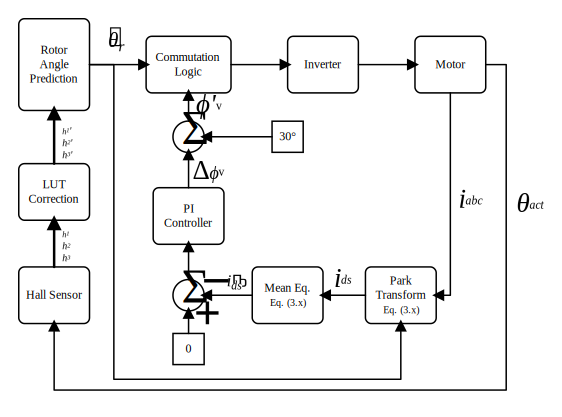
\includegraphics[width=0.9\columnwidth, page=1]{figures/Visio/Flowcharts_1.pdf}
    \caption{Flowchart of the MTPA PI controller. The corrected Hall signals provide accurate $\hat{\theta}_r$ for computing $i_{ds}$ from phase currents. The average $\bar{i}_{ds}$ is fed to the PI controller, which outputs compensation angle $\Delta\phi_v$ to maintain MTPA.}
    \label{fig:mtpa_diagram}
\end{figure}

The total firing angle combines the COM advance with the dynamic compensation:
\begin{equation}
    \phi'_v[n] = 30° + \Delta \phi_v[n]
    \label{eq:total_firing_angle}
\end{equation}

This corrected angle $\phi'_v$ adjusts when the VSI commutates relative to Hall transitions. At higher speeds, 
the inductive lag increases due to the rotational coupling term $\omega_r L_s i_q$ in \eqref{eq:vd}, 
requiring larger $\Delta\phi_v$. Similarly, at higher torque (larger $i_q$), the current rise time during 
commutation is longer, also requiring more advance. 
By using PI controller, the system can automatically find the 
optimal $\Delta\phi_v$ for each operating point for MTPA operation.

Together with the LUT-based Hall correction from Section \ref{sec:hall_filter}, this combined control architecture \cite{b1} enables BLDC motors with Hall sensor misalignment and large stator inductance to achieve near-optimal MTPA operation. The commutation timing is influenced by both corrections:
\begin{equation}
    t_{out}(n) = t_{in}(n) + \tau_{corr}(n) - \frac{\Delta\phi_v[n]}{\hat{\omega}_r[n]}
    \label{eq:combined_timing}
\end{equation}
where the first correction term $\tau_{corr}(n)$ from \eqref{eq:tau_lut} balances the Hall intervals, and the second term applies the MTPA advance compensation. 
The system dynamically adjusts both corrections in real time to maintain optimal performance.



\section{Detailed Machine Simulations}
\label{sec:simulation}
The proposed combined control strategy was validated using Simulink and a common industrial BLDC motor. 
The motor parameters are listed in the B.




\subsection{Validation of LUT and MTPA Controller}


To validate the effectiveness of the proposed LUT-based Hall correction and MTPA controller, we will 
compare the method against the model in past literatures \cite{b1, b2}.

First the motor is simulated with Hall sensor misalignment of $+9^{\circ}$, $-1^{\circ}$, and $+7^{\circ}$ for $H_1$, $H_2$, and $H_3$ respectively.
By running the calibration phase with the 6-step averaging filter from \eqref{eq:tau_a6},
the LUT correction angles for each sector can be visualized as shown in \Cref{fig:lut_correction_angles}. 

\begin{figure}[htbp]
    \centering
    \includegraphics[width=0.5\linewidth]{figures/lut_angle_chart.png}
    \caption{Visualised LUT correction angles for Hall sensor misalignment.}
    \label{fig:lut_correction_angles}
\end{figure}

Then, \Cref{fig:lut_vs_filter_verification} compares the behaviour of Hall correction either with LUT or filter, 
along with MTPA. 
The figure is divided into three sequential stages to illustrate the sequence of operations each controller do.
Initially, both methods start with no Hall compensation, resulting in significant oscillations in $i_d$ and $\bar{i}_d$.
Then the Hall correction is enabled either through the filter (a) or LUT (b). 
Observe that both methods successfully balance the switching intervals as indicated by the 
symmetric current waveform. Consequently, the oscillations in $i_d$ and $\bar{i}_d$ are eliminated, with $\bar{i}_d$ reaching a non zero
constant value. This confirms the validity of using LUT for Hall correction, achieving similar steady-state performance as the filter method
in past studies.
%% FIX needs to be moved up to make it look good
\begin{figure}[htbp]
    \centering
    \includegraphics[width=\linewidth]{figures/current_transient_stacked_inset.png}
    \caption{Simulated phase current $i_{a}$, d-axis current $i_{d}$, and time averaged d-axis current $i_{\bar{d}}$ for (a) Filter, (b) MTPA.}
    \label{fig:lut_vs_filter_verification}
\end{figure}
\Cref{fig:lut_vs_filter_verification}


Since the $\bar{i}_d$ is now stable, it is now suitable for MTPA control. Note that after the MTPA is activated, 
the PI controller quickly drives $\bar{i}_d$ to zero, achieving MTPA operation. From \Cref{sec:mtpa_control} 
we can verify the effectiveness of the MTPA by observing the alignment of phase currents and back-EMF. 

\begin{figure}[htbp]
\centerline{\includegraphics[width=\columnwidth]{figures/1_phase_alignment.png}}
\caption{Alignment of the fundamental phase current and back-EMF: (a) uncompensated; (b) LUT only; (c) LUT + MTPA controller.}
\label{fig:alignment}
\end{figure}

\Cref{fig:alignment} compares the uncompensated case (a), the LUT-only case (b), and the combined Method (c). 
The uncompensated waveforms show significant distortion and phase lag. The filter balances the switching intervals, 
but the phase lag persists. Finally, combining the LUT with MTPA (c), the controller achieves both balanced intervals 
and aligns the fundamental phase current and back-EMF and we achieve MTPA operation.


\Cref{fig:results_torque} presents the steady-state performance comparison in terms of torque generation efficiency, 
defined as the ratio of average torque to RMS phase current ($K_t = \bar{T}_e / I_{rms}$). 
The uncompensated case exhibits the lowest efficiency due to significant phase misalignment. 
The filter-only approach improves commutation symmetry but introduces delays that prevent optimal 
torque production. The proposed combined method (LUT + MTPA) demonstrates the highest torque-per-ampere ratio, 
confirming that the algorithm successfully compensates for both Hall sensor placement errors and inductive phase 
lag, thereby recovering the optimal operating point.

\begin{figure}[htbp]
\centerline{\includegraphics[width=\columnwidth]{figures/2_tpa_comparison.png}}
\caption{Comparison of Torque Generation Efficiency (Torque Constant $K_t$). The proposed LUT + MTPA method achieves the highest 
torque-per-ampere, indicating optimal alignment.}
\label{fig:results_torque}
\end{figure}

\subsection{Transient Performance}

% \Cref{fig:speed_step} illustrates the speed response of the motor to a step command. The yellow trace representing the proposed LUT correction demonstrates a response time comparable to the ideal sensor placement (blue trace), significantly outperforming the 3-step and 6-step averaging filters which introduce noticeable delays and overshoot.

% \begin{figure}[htbp]
% \centerline{\includegraphics[width=\columnwidth]{figures/speed_step_placeholder.png}}
% \caption{Simulated speed response step increase. (a) with ideal Hall sensor placement; (b) Comparison of averaging filters vs. proposed LUT correction. The LUT method achieves faster convergence.}
% \label{fig:speed_step}
% \end{figure}

\Cref{fig:startup} illustrates the speed response of the motor when applying the filter from startup. 
As shown, the proposed LUT correction achieves a response time comparable to the ideal sensor placement and the Hall intervals are corrected from startup. 
In contrast, the 3-step and 6-step averaging filters due to their memory based nature, was not able to be properly initialized from startup.
Filter based approach needs to wait for the motor to reach steady state before they can be activated, where as LUT approach can be used immediately after the calibration.
This demonstrates the advantage of the LUT method in better transient performance.
\begin{figure}[htbp]
\centerline{\includegraphics[width=\columnwidth]{figures/3_startup.png}}
\caption{Simulated speed response step increase. (a) with ideal Hall sensor placement; (b) Comparison of averaging filters vs. proposed LUT correction. The LUT method achieves faster convergence.}
\label{fig:startup}
\end{figure}

\Cref{fig:load_step} depicts the system response to a sudden load torque step. The performances are similar. 
% The LUT-based controller maintains stability and exhibits superior torque dynamic performance. 
% The speed dip is minimized, and the electromagnetic torque recovers smoothly without the oscillatory 
% behavior observed in the conventional averaging methods.

\begin{figure}[htbp]
\centerline{\includegraphics[width=\columnwidth]{figures/4_torque_step.png}}
\caption{Simulated response to a load step increase: (a) speed response; (b) electromagnetic torque response. The proposed LUT correction (yellow trace) shows superior dynamic tracking.}
\label{fig:load_step}
\end{figure}

\section{Conclusion}
\label{sec:conclusion}
This paper presented a unified control framework addressing two critical performance bottlenecks in BLDC drives: sensor misalignment and inductive lag. 
By integrating a LUT-based calibration with a dynamic MTPA controller, the system achieves smooth and efficient operation. 
Simulation results confirm the method's ability to eliminate misalignment in Hall sensor signals and achieving 
maximum torque-per-ampere (MTPA) operation, while maintaining excellent transient 
response characteristics suitable for dynamic industrial applications. Future research will
explore experimental validation through microcontroller implementation.

\appendix[Motor Parameters]
The main parameters of the BLDC motor used in this study are listed in Table \ref{tab:motor_params}.
\begin{table}[htbp]
\caption{Motor Parameters}
\begin{center}
\begin{tabular}{|c|c|c|}
\hline
\textbf{Parameter} & \textbf{Symbol} & \textbf{Value} \\
\hline
Stator Resistance & $R_s$ & \SI{0.5}{\ohm} \\
\hline
Stator Inductance & $L_s$ & \SI{1.2}{mH} \\
\hline
Flux Linkage & $\psi_m$ & \SI{0.05}{Wb} \\
\hline
Pole Pairs & $P$ & 4 \\
\hline
Rated Speed & $\omega_{rated}$ & \SI{3000}{rpm} \\
\hline
\end{tabular}
\label{tab:motor_params}
\end{center}
\end{table}

\appendix[PI Controller Gains]
\label{sec: PI_gains}
The PI controller gains used in the MTPA control are listed in Table \ref{tab:pi_gains}.
\begin{table}[htbp]
\caption{PI Controller Gains}
\begin{center}
\begin{tabular}{|c|c|}
\hline
\textbf{Gain} & \textbf{Value} \\
\hline
Proportional Gain & $K_p = 0.0068$ \\
\hline
Integral Gain & $K_i = 0.744$ \\
\hline
\end{tabular}
\label{tab:pi_gains}
\end{center}
\end{table}

\section*{Acknowledgment}
The authors acknowledge the support of the Department of Electrical and Computer Engineering at the University of British Columbia.

\begin{thebibliography}{00}

\bibitem{b1} M. Phung, ``Maximum Torque per Ampere Control of Brushless DC Motors with Large Winding Time Constant and Hall-Sensor Misalignment,'' B.A.Sc. thesis, University of British Columbia, Vancouver, BC, Canada, 2025.
\bibitem{b2} M. Hasman, ``Mitigating Misaligned Hall Sensors in Brushless DC Motors Using a Calibration Routine for Improved Fast Electromechanical Transients,'' B.A.Sc. thesis, University of British Columbia, Vancouver, BC, Canada, 2025.
\bibitem{b3} P. C. Krause, O. Wasynczuk, S. D. Pekarek, and T. O'Connell, \emph{Electromechanical Motion Devices: Rotating Magnetic Field-based Analysis with Online Animations}. Hoboken, NJ, USA: Wiley-IEEE Press, 2020.
\bibitem{b4} P. Pillay and R. Krishnan, ``Modeling, simulation, and analysis of permanent-magnet motor drives, part II: The brushless DC motor drive,'' \emph{IEEE Trans. Ind. Appl.}, vol. 25, no. 2, pp. 265--273, Mar./Apr. 1989.
\bibitem{b5} S. D. Sudhoff and P. C. Krause, ``Operating modes of the brushless DC motor with a 120 degrees inverter,'' \emph{IEEE Trans. Energy Convers.}, vol. 5, no. 3, pp. 558--564, Sep. 1990.
\bibitem{b6} N. Samoylenko, Q. Han, and J. Jatskevich, ``Dynamic Performance of Brushless DC Motors With Unbalanced Hall Sensors,'' \emph{IEEE Trans. Energy Convers.}, vol. 23, no. 3, pp. 752--763, Sep. 2008.
\bibitem{b7} P. Alaeinovin, S. Chiniforoosh, and J. Jatskevich, ``Evaluating misalignment of hall sensors in brushless DC motors,'' in \emph{Proc. IEEE Canada Electr. Power Conf.}, Oct. 2008, pp. 1--6.
\bibitem{b8} J. Zhou, S. Ebrahimi, and J. Jatskevich, ``Extended Operation of Brushless DC Motors Beyond 120$^{\circ}$ under Maximum Torque Per Ampere Control,'' \emph{IEEE Trans. Energy Convers.}, vol. 38, no. 2, pp. 1--12, Jun. 2023.
\bibitem{b9} P. Alaeinovin and J. Jatskevich, ``Filtering of Hall-Sensor Signals for Improved Operation of Brushless DC Motors,'' \emph{IEEE Trans. Energy Convers.}, vol. 27, no. 2, pp. 547--549, Jun. 2012.
\bibitem{b10} J. Zhou, J. Lu, S. Ebrahimi, and J. Jatskevich, ``A Compensation of Commutation Angle in Hall-Sensor-Controlled Brushless DC Motors for Maximum Torque per Ampere Operation,'' in \emph{Proc. 21st Int. Symp. INFOTEH-JAHORINA}, Mar. 2022, pp.
\bibitem{b11} B. Tan, X. Wang, D. Zhao, K. Shen, J. Zhao, and X. Ding, ``A Lag Angle Compensation Strategy of Phase Current for High-Speed BLDC Motors,'' \emph{IEEE Access}, vol. 7, pp. 9566--9574, 2019.
\bibitem{b12} X. Shi, X. Wang, C. Gu, and Z. Deng, ``A novel commutation correction method for high-speed PM brushless dc motor,'' in \emph{Proc. IEEE Appl. Power Electron. Conf. Expo. (APEC)}, Mar. 2017, pp. 1899--1905.
\bibitem{b13} The MathWorks, Inc., \emph{SimPowerSystems: Model and Simulate Electrical Power Systems User's Guide}. Natick, MA, USA: The MathWorks, Inc., 2006.

\end{thebibliography}

\end{document}
